\chapter{Data storage}
Data storage is important in a system like a windmill farm.
A lot of data must be persisted like weather data, health data of the different parts of every turbine and production data.
These records are important both for immediate use to view the current state of the system but also for review in the future for instance to predict weather trends or replace worn down parts of turbine before they break completely.

Currently data is aggregated from each turbine and stored on a central node.
This node will over time aggregate hundreds of gigabytes of information.
The data on the node is secured by backup but it is still a single point of failure.
Take out the data storage node or the communication to it and a lot of information will be lost.

By distributing the data of the system between all the connected nodes we achieve better redundancy because the data is present on many different nodes.
Should a node become unavailable another node can communicate the same data in effect strengthening the availability of the system.

This chapter contains a description of a number of relevant storage technologies and a discussion of which technology is the best suited for a system like the Siemens case.

\section{Relational storage, SQL}
\label{sec:sql}
The traditional way of storing data is in a Relational Database Management System(RDBMS).
These databases rely on a schema to arrange data in tables and their relations.
Using SQL it is easy to query data and to do aggregate operations.
RDBMSs support ACID transactions which ensures operations in the database are processed reliably.

A shortcoming of the RDBMSs is the problem with object-relational mapping also known as the Impedance Mismatch Problem\cite{Fowler:IntroNoSQL, Neward:TheVietnamOfComputerScience}.
The relational structure of the RDBMSs does not map well to the object-oriented structure the most popular programming languages encourage.
Often an object is an aggregate of a number of attributes.
In the context of the object-oriented program the object is seen as one entity.
In the context of the RDBMS the attributes of the object-oriented object is often scattered between multiple tables in the database to ensure consistency and avoid duplicate data.
This mismatch between object representation and relational representation can cause both performance problems, the JOIN operation in SQL is very costly, as well as considerable development time spent mapping one structure to the other.
The performance problem multiplies in a distributed database if the RDBMS must do JOIN operations across the network in order to aggregate data.

Another problem with a traditional RDBMS is that they are designed for vertical scaling\cite{Atzeni:TheRelationalModelIsDead}. If a traditional RDBMS has problems handling data the solution is to add a bigger harddrive or invest in a faster CPU. This makes sense in a world were hardware is very expensive like it was when the traditional RDBMSs saw the light of day\cite{Stonebraker:TheEndOfAnArchitecturalEra}. Today horizontal scaling is preferred. If a system has a problem with the data load add another machine or add five others if that is what it takes.

\section{Schema-less storage, NoSQL}
\label{sec:nosql}
Since 2009 the schema-less storage methods have become increasingly popular.
Relational databases could no longer keep up with the task of storing and querying big data.
A new breed of schema-less storage systems became popular because they could handle some of the problems big data caused for the relational storage systems.
This new breed of databases are designed for horizontal scalability and without strict schemas allowing a more flexible data model. 
They are capable of handling huge amounts of data both for storage but also for analysis or batch operations.
The downside however is the lack of the ACID properties which results in a lower consistency and the lack of transactions. %TODO: Dårligt formuleret omskriv!

The schema-less databases can be divided roughly into four categories\cite{Fowler:IntroNoSQL, Moniruzzaman:NoSQLDatabaseNewEraOfDatabasesForBigDataAnalysis}, which will be described separately in the following sections.

\subsection{Document databases}
The document databases are designed to contain documents.
The documents contains attribute name/value pairs.
Attributes may vary between rows.
To retrieve data it is possible to search both on the attribute and the value.

Primary use include storing actual documents like emails and blog posts, or storage of semi-structured and aggregate data.

\begin{figure}
	\centering

	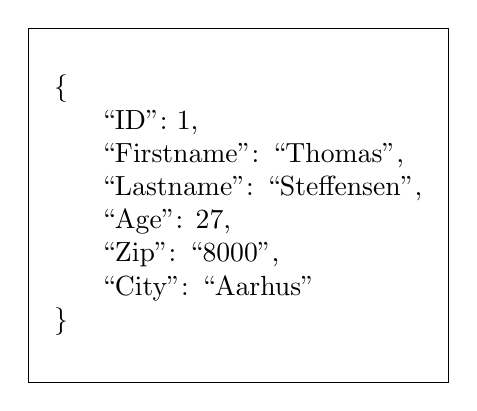
\begin{tikzpicture}
		\node[draw, rectangle, minimum height=4.5cm] (a) {
			\begin{tabular}{c l}
				\{ & \\
				& ``ID'': 1, \\
				& ``Firstname'': ``Thomas'', \\
				& ``Lastname'': ``Steffensen'', \\
				& ``Age'': 27, \\
				& ``Zip'': ``8000'', \\
				& ``City'': ``Aarhus'' \\
				\} &
			\end{tabular}};
	\end{tikzpicture}

	\captionsetup{format=plain,font=footnotesize,labelfont={bf,defaultCapFont},labelsep=quad,singlelinecheck=no}
		\caption[Document store]{
			\label{fig:DocumentStore}
			\footnotesize{%
				Document store structure.
			} 
	}
\end{figure}

% \begin{figure}
% 	\centering
% 	\includegraphics[scale=0.8]{Document.png} 
% 	\captionsetup{format=plain,font=footnotesize,labelfont={bf,defaultCapFont},labelsep=quad,singlelinecheck=no}
% 	\caption[Document store]{
% 		\label{fig:DocumentStore}
% 		\footnotesize{%
% 			Document store structure.
% 		} 
% 	}
% \end{figure}

\subsection{Key-value stores}
The key-value stores can be compared to a hashmap since every entry has a key and an associated value. 
To retrieve data you search for the key. 
The values can contain any kind of data from simple text to lists or documents.

Primary use includes fast lookup for instance for user sessions or product lists.

\begin{figure}
	\centering

	\begin{tikzpicture} [
			diagram item/.style={
				minimum width=3cm,
				minimum height=1cm,
				draw,
				rectangle
			}
		]
		\node[diagram item] (a) {Key: User1};
		\node[diagram item, right=.5cm of a] (b) {Value: Stefan};

		\node[diagram item, below=.2cm of a] (c) {Key: User2};
		\node[diagram item, right=.5cm of c] (d) {Value: Thomas};

	    \draw[arrows=->] (a) to (b);
	    \draw[arrows=->] (c) to (d);
	\end{tikzpicture}

	\captionsetup{format=plain,font=footnotesize,labelfont={bf,defaultCapFont},labelsep=quad,singlelinecheck=no}
		\caption[Key-value store]{
			\label{fig:KeyValueStore}
			\footnotesize{%
				Key-value store structure.
			} 
		}
\end{figure}

% \begin{figure}
% 	\centering
% 	\includegraphics[scale=0.8]{KeyValue.png} 
% 	\captionsetup{format=plain,font=footnotesize,labelfont={bf,defaultCapFont},labelsep=quad,singlelinecheck=no}
% 	\caption[Key-value store]{
% 		\label{fig:KeyValueStore}
% 		\footnotesize{%
% 			Key-value store structure.
% 		} 
% 	}
% \end{figure}

\subsection{Column-family stores}
Column-family stores keep related data stored together.
A column-family object consists of a key-value pair where the value contains columns of related data.

Primary use includes distributed data storage, batch processing of data and analytical processing for statistical use.

\begin{figure}
	\centering

	\begin{tikzpicture} [
			diagram item/.style={
				minimum width=3cm,
				minimum height=1cm,
				draw,
				rectangle
			},
			diagram bigitem/.style={
				minimum width=3cm,
				minimum height=2cm,
				draw,
				rectangle
			}
		]


		\node (a) {Row key};
		\node [right=5.7cm of a] (b) {Columns};
		\node[diagram bigitem, below=0cm of a] (c) {User1};
		
		%Attribute names
		\node[diagram item, right=1.5cm of c, anchor=south] (d) {Firstname};
		\node[diagram item, right=0cm of d] (e) {Lastname};
		\node[diagram item, right=0cm of e] (f) {Age};
		\node[diagram item, right=0cm of f] (g) {Zip};

		%Attribute values
		\node[diagram item, below=0cm of d] (h) {Thomas};
		\node[diagram item, below=0cm of e] (i) {Steffensen};
		\node[diagram item, below=0cm of f] (j) {27};
		\node[diagram item, below=0cm of g] (k) {8000};

		\node[diagram bigitem, below=.2cm of c] (l) {User2};
		
		%Attribute names
		\node[diagram item, right=1.5cm of l, anchor=south] (m) {Firstname};
		\node[diagram item, right=0cm of m] (n) {Zip};

		%Attribute values
		\node[diagram item, below=0cm of m] (o) {Thomas};
		\node[diagram item, below=0cm of n] (p) {8000};
	\end{tikzpicture}

	\caption[Column-family store]{
		\label{fig:ColumnFamilyStore}
		\footnotesize{%
			Column-family store structure.
		} 
	}
\end{figure}

% \begin{figure}
% 	\centering
% 	\includegraphics[scale=0.8]{ColumnFamily.png} 
% 	\captionsetup{format=plain,font=footnotesize,labelfont={bf,defaultCapFont},labelsep=quad,singlelinecheck=no}
% 	\caption[Column-family store]{
% 		\label{fig:ColumnFamilyStore}
% 		\footnotesize{%
% 			Column-family store structure.
% 		} 
% 	}
% \end{figure}

\subsection{Graph databases}
Graph databases divides data according to nodes and relations between nodes.
Each node in the graph contains key-value pairs of data, and each edge describes a relationship to another node.
Graph databases are optimized for traversal of relationships between nodes, not for data aggregation or analysis.

Primary use includes pattern detection and mapping of networks.

\begin{figure}
	\centering
	\begin{tikzpicture} [
			diagram item/.style={
				minimum width=5.3cm,
				minimum height=1.5cm,
				draw,
				rectangle
			}
		]

		\node[diagram item] (a) {
			\begin{tabular}{rl}
				Firstname:&Thomas \\
				Lastname:&Steffensen
			\end{tabular}};

		\node[diagram item, right=3 of a] (b) {
			\begin{tabular}{rl}
				Firstname:&Stefan \\
				Age:&27
			\end{tabular}};

		\node[diagram item, below=3 of a] (c) {
			\begin{tabular}{rl}
				Firstname:&Mette \\
				Occupation:&Student
			\end{tabular}};

		\node[diagram item, right=3 of c] (d) {
			\begin{tabular}{rl}
				Name:&Aarhus Universitet
			\end{tabular}};

		\path (a) -- node[sloped] (knows) {knows} (b);
		\path (a) -- node[sloped] (married) {married to} (c);
		\path (a) -- node[sloped] (studies1) {studies at} (d);
		\path (b) -- node[sloped] (studies2) {studies at} (d);

	    \draw[->] (a)--(knows)--(b);
	    \draw[->] (a)--(married)--(c);
	    \draw[->] (a)--(studies1)--(d);
	    \draw[->] (b)--(studies2)--(d);
	\end{tikzpicture}
\end{figure}

% \begin{figure}
% 	\centering
% 	\includegraphics[scale=0.8]{Graph.png} 
% 	\captionsetup{format=plain,font=footnotesize,labelfont={bf,defaultCapFont},labelsep=quad,singlelinecheck=no}
% 	\caption[Graph store]{
% 		\label{fig:GraphStore}
% 		\footnotesize{%
% 			Graph store structure.
% 		} 
% 	}
% \end{figure}

\section{Relational storage that scale, NewSQL}
\label{sec:newsql}
NewSQL data stores aim to bring the relational data model into the world of horizontal scalability and flexible data models while maintaining the ACID properties and transactions of the traditional RDBMS\cite{Cattell:ScalableSQLAndNoSQLDataStores}.
This is obtained by implementing a completely new architecture\cite{CORBETT:SpannerGooglesGloballyDistributedDatabase}.
Starting from nothing with a new architecture allows the NewSQL data stores to be designed to take advantage of the distributed paradigms and to incorporate more flexibility into the schema structure.
The key differences between traditional SQL data stores and the NewSQL data stores are therefore found in the way the NewSQL data stores are built for scalability and performance.
They try to avoid the major performance barriers which are locking, write-ahead logging, buffer pool overhead and latching\cite{Stonebraker:NewSQLvsNoSQLForNewOLTP}.

Locking can be avoided by performing transactions in timestamp order or using multi version concurrency control.
Write-ahead logging can be avoided by doing automatic replication and failover.
To avoid buffer pool overhead the NewSQL data stores can run in main memory, either entirely or have a hot store in memory for active data and a cold store on disk for stale data.
To avoid latching transactions can be run single-threaded, meaning transactions must run to completion without descheduling.

Using some or all of these performance upgrades the NewSQL data stores can achieve higher performance than the traditional SQL data stores.
Other features like distributed concurrency control and distributed query processing allows the NewSQL data stores to scale horizontally.

NewSQL data stores are divided into three categories\cite{Prasanns:NewSQLTheNewWayToHandleBigData}:

\begin{itemize}
\item New databases: Completely new systems designed for scalability and performance.
\item New MySQL storage engine: Keep the existing MySQL interface and redesign the storage engine in order to achieve scalability.
\item Transparent clustering/sharding: Provide extra features for transparent clustering/sharding on top of existing database systems. 
\end{itemize}

\section{SQL, NoSQL or NewSQL?}
This thesis aims to create a distributed system with scalability and redundancy as the most important parameters.
This means that traditional SQL is not an option because of the poor scalability.

NoSQL and NewSQL has clear advantages because they are built as a consequence of the shortcomings of the traditional database systems when it comes to distributed systems.
NoSQL has the advantage of high scalability and high performance on data analysis, but the cost is a lack of ACID and transactions.
NewSQL promises to keep the virtues of the traditional databases systems while simultaneously allowing horizontal scalability and high performance.

Since both NoSQL and NewSQL seems like fitting technologies for data management in the Siemens case a further comparison between two state of the art implementations must be done in order to decide which technology will be the best suited.

\section{State of the art NoSQL and NewSQL}
To identify state of the NoSQL and NewSQL databases a website called db-engines.com\cite{db-engines} is used. This website maintain a list of more than 200 different databases ranked by popularity. The list is updated monthly based on search engine popularity, discussion threads, job-offers, mentions on LinkedIn and tweets. This does not give the complete and objective ranking but it gives a pointer to the most popular items in their respective category.

\section{Comparison of MongoDB and VoltDB}

\section{Conclusion}